%!TEX program = xelatex
\documentclass[dvipsnames, svgnames,a4paper,11pt]{article}
% ----------------------------------------------------- 
%	加边框的命令
%	参考:https://tex.stackexchange.com/questions/531559/how-to-add-the-page-border-for-first-two-pages-in-latex
\usepackage{tikz}
\usetikzlibrary{calc}
\usepackage{eso-pic}
\AddToShipoutPictureBG{%
\begin{tikzpicture}[overlay,remember picture]
\draw[line width=0.6pt] % 边框粗细
    ($ (current page.north west) + (0.6cm,-0.6cm) $)
    rectangle
    ($ (current page.south east) + (-0.6cm,0.6cm) $); % 边框位置
\end{tikzpicture}}


\usepackage{xcolor}
\definecolor{c1}{HTML}{070F94} % 目录颜色 原版为2752C9 紫灰色535AAA 蓝紫色0B0DB7 深蓝色070F94 湖绿色219394 松石灰绿086173
\definecolor{c2}{HTML}{E20129} % 引用颜色 原版\definecolor{c2}{RGB}{190,20,83} 橙色F24729

\usepackage{ctex}
\usepackage[top=28mm,bottom=28mm,left=15mm,right=15mm]{geometry}
\usepackage{hyperref} 
\hypersetup{
	colorlinks,
	linktoc = section, % 超链接位置,选项有section, page, all
	linkcolor = c1, % linkcolor 目录颜色
	citecolor = c1  % citecolor 引用颜色
}
\usepackage{amsmath,enumerate,multirow,float}
\usepackage{tabularx}
\usepackage{tabu}
\usepackage{subfig}
\usepackage{fancyhdr}
\usepackage{graphicx}
\usepackage{wrapfig}  
\usepackage{physics}
\usepackage{appendix}
\usepackage{amsfonts}

%
\usepackage{tcolorbox}
\tcbuselibrary{skins,breakable}
\newtcolorbox{tbox}[2][]{
    colframe=black!70!,
    breakable,
    enhanced,
	boxrule =0.5pt,
    title = {#2},
    fonttitle = \large\kaishu\bfseries,
	drop fuzzy shadow,
    #1
}
\newtcolorbox[auto counter,number within=section]{question}[1][]{
  top=2pt,bottom=2pt,arc=1mm,
  boxrule=0.5pt,
%   frame hidden,
  breakable,
  enhanced, %跨页后不会显示下边框
  coltitle=c1!80!gray,
  colframe=c1,
  colback=c1!3!white,
  drop fuzzy shadow,
  title={思考题~\thetcbcounter:\quad},
  fonttitle=\bfseries,
  attach title to upper,
  #1
}

% ---------------------------------------------------------------------
%	利用cleveref改变引用格式,\cref是引用命令
\usepackage{cleveref}
\crefformat{figure}{#2{\textcolor{c2}{Figure #1}}#3} % 图片的引用格式
\crefformat{equation}{#2{(\textcolor{c2}{#1})}#3} % 公式的引用格式
\crefformat{table}{#2{\textcolor{c2}{Table #1}}#3} % 表格的引用格式


% ---------------------------------------------------------------------
%	页眉页脚设置
\fancypagestyle{plain}{\pagestyle{fancy}}
\pagestyle{fancy}
\lhead{\kaishu 中山大学物理与天文学院基础物理实验\uppercase\expandafter{\romannumeral2}} % 左边页眉,学院 + 课程
\rhead{\kaishu 实验报告By黄罗琳} % 右边页眉,实验报告标题
\cfoot{\thepage} % 页脚,中间添加页码


% ---------------------------------------------------------------------
%	对目录、章节标题的设置
\renewcommand{\contentsname}{\centerline{\huge 目录}}
\usepackage{titlesec}
\usepackage{titletoc}
% \titleformat{章节}[形状]{格式}{标题序号}{序号与标题间距}{标题前命令}[标题后命令]
\titleformat{\section}{\centering\LARGE\songti}{}{1em}{}

% ---------------------------------------------------------------------
%   listing代码环境设置
\usepackage{listings}
\lstloadlanguages{python}
\lstdefinestyle{pythonstyle}{
backgroundcolor=\color{gray!5},
language=python,
frameround=tftt,
frame=shadowbox, 
keepspaces=true,
breaklines,
columns=spaceflexible,                   
basicstyle=\ttfamily\small, % 基本文本设置,字体为teletype,大小为scriptsize
keywordstyle=[1]\color{c1}\bfseries, 
keywordstyle=[2]\color{Red!70!black},   
stringstyle=\color{Purple},       
showstringspaces=false,
commentstyle=\ttfamily\scriptsize\color{green!40!black},%注释文本设置,字体为sf,大小为smaller
tabsize=2,
morekeywords={as},
morekeywords=[2]{np, plt, sp},
numbers=left, % 代码行数
numberstyle=\it\tiny\color{gray}, % 代码行数的数字字体设置
stepnumber=1,
rulesepcolor=\color{gray!30!white}
}




% ---------------------------------------------------------------------
%	其他设置
\def\degree{${}^{\circ}$} % 角度
\graphicspath{{./images/}} % 插入图片的相对路径
\allowdisplaybreaks[4]  %允许公式跨页 
\usepackage{lipsum}
\usepackage{adjustbox}
%\usepackage{mathrsfs} % 字体
%\captionsetup[figure]{name=Figure} % 图片形式
%\captionsetup[table]{name=Table} % 表格形式
\begin{document}
	
	% 实验报告封面	
	% 顶栏
	\begin{table}
		\renewcommand\arraystretch{1.7}
		\begin{tabularx}{\textwidth}{
				|X|X|X|X
				|X|X|X|X|}
			\hline
			\multicolumn{2}{|c|}{预习报告}&\multicolumn{2}{|c|}{实验记录}&\multicolumn{2}{|c|}{分析讨论}&\multicolumn{2}{|c|}{总成绩}\\
			\hline
			\LARGE25 & & \LARGE25 & & \LARGE30 & & \LARGE80 & \\
			\hline
		\end{tabularx}
	\end{table}
	% ---
	
	% 信息栏
	\begin{table}
		\renewcommand\arraystretch{1.7}
		\begin{tabularx}{\textwidth}{|X|X|X|X|}
			\hline
			年级、专业: & 2022级 物理学 &组号: & 实验组1\\
			\hline
			姓名: & 黄罗琳   & 学号: &22344001   \\
			\hline
			实验时间: & 2024/4/11 & 教师签名: & \\
			\hline
		\end{tabularx}
	\end{table}
	% ---
	
	% 大标题
	\begin{center}
		\LARGE CB2  \quad 偏振光实验
	\end{center}
	% ---
	
	% 注意事项
	
	% 基本
	\textbf{【实验报告注意事项】}
	\begin{enumerate}
		\item 实验报告由三部分组成:
		\begin{enumerate}
			\item 预习报告:课前认真研读实验讲义,弄清实验原理;实验所需的仪器设备、用具及其使用、完成课前预习思考题;了解实验需要测量的物理量,并根据要求提前准备实验记录表格(可以参考实验报告模板,可以打印)。\textcolor{red}{\textbf{(20分)}}
			\item 实验记录:认真、客观记录实验条件、实验过程中的现象以及数据。实验记录请用珠笔或者钢笔书写并签名(\textcolor{red}{\textbf{用铅笔记录的被认为无效}})。\textcolor{red}{\textbf{保持原始记录,包括写错删除部分,如因误记需要修改记录,必须按规范修改。}}(不得输入电脑打印,但可扫描手记后打印扫描件);离开前请实验教师检查记录并签名。\textcolor{red}{\textbf{(30分)}}
			\item 数据处理及分析讨论:处理实验原始数据(学习仪器使用类型的实验除外),对数据的可靠性和合理性进行分析;按规范呈现数据和结果(图、表),包括数据、图表按顺序编号及其引用;分析物理现象(含回答实验思考题,写出问题思考过程,必要时按规范引用数据);最后得出结论。\textcolor{red}{\textbf{(30分)}}
		\end{enumerate}
		\textbf{实验报告就是将预习报告、实验记录、和数据处理与分析合起来,加上本页封面。\textcolor{red}{(80分)}}
		\item 每次完成实验后的一周内交\textbf{实验报告}
		
	\end{enumerate}
	
	% 安全
	\textbf{【实验安全注意事项】}	
	\begin{enumerate}
		\item 实验中不要用手触摸镜片,以免弄脏镜片;
		\item 避免直视光源,注意光源表面高温;
		\item 注意用电安全。
		
	\end{enumerate}
	
	% 目录
	\clearpage
	\tableofcontents
	\clearpage
	% ---
	
	
	
	% 预习报告	
	
	% 小标题
	\setcounter{section}{0}
	\section{CB2 偏振光实验 \quad\heiti 预习报告}
	% ---
	
	% 实验目的
	\subsection{实验目的}
	\begin{enumerate}
		\item 理解偏振光的基本概念,了解线偏振光、椭圆偏振光和圆偏振光。
		\item 分析偏振光产生的三种方法:吸收、反射和散射。
		\item 了解在各向异性材料介质中光波的传播,学习偏振光通过各向异性介质后,产生的“相位延迟”($\lambda/2$ 波片和 $\lambda/4$ 波片)。
	\end{enumerate}
	% ---
	
	% 仪器用具
	\subsection{仪器用具}
	\begin{table}[htbp]
		\centering
		\renewcommand\arraystretch{1.6}
		\begin{tabular}{c|c|c|p{0.5\textwidth}}
			\hline
			\textbf{编号} & \textbf{仪器用具名称} & \textbf{数量} & \textbf{主要参数(型号,测量范围,测量精度等)} \\
			\hline
			1 & 光功率计 & 1 & \\
			2 & 白光光源 &  & \\
			3 & 光学导轨 &  & \\
			4 & 光学测角台 &  & \\
			5 & 偏振片 & 3 & \\
			6 & 半波片 & 1 & \\
			7 & 1/4 波片 & 2 & \\
			\hline
		\end{tabular}
	\end{table}
	% ---
	
	% 原理概述
	\subsection{原理概述}
{ \textbf{\large {偏振光的产生}} }

(1) 偏振片的工作原理
偏振片的工作原理是对光在偏振方向具有选择性吸收。理想情况下,在特定的方向透过线性偏振光(称为透振方向),吸收与透振方向成正交方向的线性偏振光。

偏振片内部的微观结构使其能够选择性地吸收特定方向的光。这种结构使得偏振片在一个方向上对光具有透明度,而在垂直方向上具有吸收性。

(2) 偏振片的微观结构
偏振片的各向异性性质主要是因为在一个方向上排列的长链形分子结构的存在下,吸收沿这个方向的偏振光。为了避免理解错误,不在这里讨论波长在光吸收现象的重要性。实验中使用的偏振片在红外光谱范围内的响应较差,但是使用的白光(灯丝)在红外区的发射不可忽略。

(3) 马吕斯定律
强度为$I_0$的线偏振光,透过检偏片后,透射光的强度(不考虑吸收)为$I = I_0\cos^2\theta$,其中$\theta$是入射线偏振光的光振动方向和偏振片透振方向之间的夹角。

马吕斯定律描述了透过偏振片的偏振光强度与入射光偏振方向与偏振片透振方向之间夹角的关系。这意味着透过偏振片的光的强度取决于入射光的偏振方向与偏振片的透振方向之间的夹角。

(4) 玻璃反射起偏
当入射光线以布儒斯特角入射时,反射光通过介质(玻璃、塑料等)是垂直于入射面的线性偏振光。定义$\theta_B$为布儒斯特角:$\tan\theta_B = \frac{n_{\text{ver}}}{n_{\text{air}}}.$ 

玻璃表面上的反射会导致反射光变成线性偏振光。这种现象发生在入射光以特定角度(布儒斯特角)进入玻璃表面时。在这个角度下,平行于入射面的电场分量不会产生反射,因此反射光成为线性偏振光,垂直于入射面。

(5) 散射起偏
当散射微粒的大小小于光波波长(波长$\lambda$)时可被视为产生瑞利散射。瑞利散射的电磁辐射功率$P_{\text{ray}}$,其中$P_{\text{ray}} \propto \lambda^{-4}$. 因此,“蓝”光散射比“红”光更强烈。

当光线遇到小于其波长的微小颗粒时,会发生散射。这种散射称为瑞利散射。由于瑞利散射的强度与波长的四次方成反比关系,因此对于蓝色光而言,其散射强度比红色光更高。\\
\indent{ \textbf{\large {各向异性介质中的光传播}} }

(1) 在线性各向异性介质中的光传播:
晶体表现出双折射现象,即折射率依赖于光波的偏振方向,因此它们是各向异性的。当光线通过均匀各向异性的线性介质时,会分解成两束偏振方向互相垂直、折射角不同的光束,它们的折射率分别为 $n_x$ 和 $n_y$。这种现象称为双折射,在各种晶体中普遍存在。

当光线入射时,考虑沿两个方向的相位速度($c_x$ 和 $c_y$),其中 $c_x \equiv n c_{0x}$,$c_y \equiv n c_{0y}$,$c_0$ 是真空中平面波的传播速度。光在传播速度较慢的轴上称为寻常光($O_x$ 轴),而在传播速度较快的轴上称为非常光($O_y$ 轴)。一束折射光遵循普通的折射定律,称为普通光(或 $o$ 光);另一束不遵循普通折射定律,称为非常光(或 $e$ 光)。$o$ 光和 $e$ 光都是偏振光,且两光束的振动方向相互垂直。

(2) 各向异性介质中的偏振:
在各向异性介质中,光程差表示为 $\delta = (n_x - n_y) e$。

(3) $\lambda/2$ 波片:
$\lambda/2$ 波片的厚度 $e$ 确保对于给定波长 $\lambda$ 的平行光正入射波晶片时,$o$ 光和 $e$ 光的光程差为 $\delta = \lambda/2$,即 $(n_x - n_y) e = \lambda/2$。

此外,$\lambda/2$ 波片只对特定波长的光通过有效。
\begin{itemize}
    \item 经过 $\lambda/2$ 波片的线偏振光仍然是线偏振光,但相对于 $O$ 轴或 $E$ 轴对称。
    \item 平行于 $O$ 轴或 $E$ 轴入射的偏振光,经过 $\lambda/2$ 波片后方向保持不变。
    \item $\lambda/2$ 波片将椭圆偏振光变为椭圆偏振光,但是改变旋转方向,使旋转方向相反。
\end{itemize}

(4) $\lambda/4$ 波片:
$\lambda/4$ 波片的厚度 $e$ 确保对于给定波长 $\lambda$ 的平行光正入射波晶片时,$o$ 光和 $e$ 光的光程差为 $\delta = \lambda/4$,即 $(n_x - n_y) e = \lambda/4$,对应相位差 $\Delta\phi = 2\pi \times \lambda/4 = \pi/2$。

另外,$\lambda/4$ 波片只对特定波长的光通过有效。
\begin{itemize}
    \item 两个 $\lambda/4$ 波片相平行,当两个波片的快慢轴一致时,相当于一个 $\lambda/2$ 波片;当一个波片的快轴与另一个波片的慢轴重合时,表现为一个各向同性波片。
    \item 椭圆偏振光经过 $\lambda/4$ 波片(波片的 $O$ 轴或 $E$ 轴与椭圆主轴一致)后成为线偏振光。
\end{itemize}

	% ---
	
	
	
	% 实验前思考题
	\subsection{实验预习题}
	
	% 思考题1
	\begin{question}
		什么是瑞利散射?
	\end{question}
	瑞利散射是一种光在遇到比其波长更小的微小颗粒(比如空气中的气体分子或水中的悬浮微粒)时发生的散射现象。在瑞利散射中,入射光波与微粒相互作用后,散射光的强度与入射光的波长的四次方成反比关系。


	% 思考题2
	\begin{question}
		举例说明瑞利散射
	\end{question}
	瑞利散射最常见于大气中,导致了蓝天的颜色。大气中的氧气和氮气分子的大小比可见光的波长小得多,因此它们会导致入射太阳光的散射,使得天空呈现出蓝色。这是因为蓝光的波长较短,散射强度更高,而红光的波长较长,散射强度相对较低,因此在观察天空时,我们会看到蓝色。

夕阳和黎明的颜色:在日出和日落时,太阳光经过较长的大气路径穿过大气层,这使得更多的光被散射,尤其是红光。因此,当我们观察日出或日落时,我们会看到天空和云彩呈现出橙色、红色或粉红色的色彩。

远处山脉的颜色:当我们观察远处的山脉或山脉的轮廓时,由于大气中的瑞利散射,远处的景物会呈现出蓝色或紫色的色调。

水中的蓝色:当我们观察清澈的水体时,水体呈现出蓝色。这是因为水分子对蓝色光的散射较强,导致我们看到水呈现出蓝色。

冰川和冰块的颜色:由于冰晶的微小结构,冰块和冰川在阳光照射下会呈现出蓝色的色调。这是因为冰晶对蓝光的瑞利散射效应导致的。

	
	% ---
	
	
	
	% 实验记录	
	\clearpage
	
	% 顶栏
	\begin{table}
		\renewcommand\arraystretch{1.7}
		\centering
		\begin{tabularx}{\textwidth}{|X|X|X|X|}
			\hline
			专业: & 物理学 & 年级: & 2022级 \\
			\hline
			姓名: & 黄罗琳& 学号: & 22344001\\
			\hline
			室温: & 23℃ & 实验地点: & A510 \\
			\hline
			学生签名:& 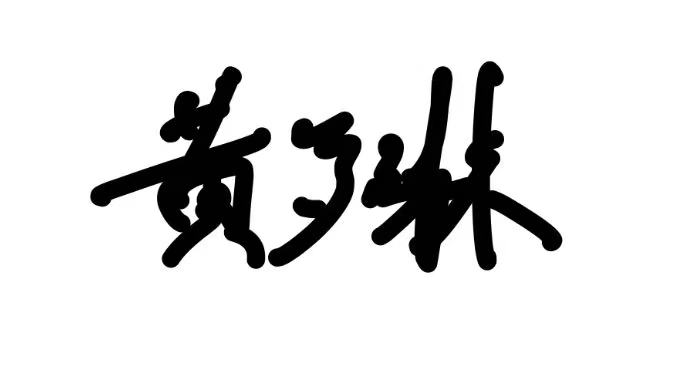
\includegraphics[width=1cm]{签字.jpg} & 评分: &\\
			\hline
			实验时间:& 2024/4/11 & 教师签名:&\\
			\hline
		\end{tabularx}
	\end{table}
	% ---
	
	% 小标题
	\section{CB2 偏振光实验 \quad\heiti 实验记录}
	% ---
	
	% 实验过程记录
	\subsection{实验内容、步骤与结果}
	
	%
	\subsubsection{研究交叉线性偏振片}
	\begin{enumerate}
	\item 实验器材:白光光源, 凸透镜, 可变光阑,两个线性偏振片,光学导轨, 屏幕。
	\item 实验步骤:
	\begin{enumerate}
		\item 用自准直等快速方法产生准直光束。
		\item 放置第一个偏振片(P1)并改变透振方向。观察屏幕上的光线强度。总结白光发出的自然光的性质。
    
    \item 放置第二个偏振片(P2)。旋转P2,改变透振方向,观察屏幕上光强的变化。发现光两次出现消失的现象,确定消光的位置。这时两个偏振片透振方向相垂直。同样的,旋转偏振片P1,能得到同样的结果。
    
    \item 在消光的位置,将P1轴旋转20°,证明P2轴旋转同样的角度时,消光现象再次出现。
    
    \item 在偏振片P1和P2之间放置第3个偏振片P3。先确定P3的透振方向,再转45°的角度,观察并说明现象。
    
    \item 拿走偏振片P3,在P1和P2之间插入塑料板或三角尺等透明物体,观察现象;转动其中任何一个元件,观察现象;给塑料板加力,观察并说明这三个现象的变化。
	\end{enumerate}	
	\item 实验数据与现象(编号与实验步骤中一致)
	 \begin{enumerate}
		\item 所用透镜焦距$f =  mm$
		\item 观察屏幕上的光线强度,光强不变,说明白光发出的自然光为随机偏振光。
		\item 设置$p_1=0°$ $p_2=   °$ 时消光\\
		设置$p_2=0°$ $p_1=   °$ 时消光
		\item 在消光的位置,将P1轴旋转20°,证明P2轴旋转20°,消光现象再次出现。
		\item P3 位置为  时消光,故 P3的透振方向为 。将 P3 旋转 45°,观察到光斑亮度减弱。
		\item 拿走偏振片 P3,在 P1 和 P2 之间插入塑料板,发现。转动其中任意一个元件,
	\end{enumerate}
	
\end{enumerate}	
	\subsubsection{验证马吕斯定律}
	\begin{enumerate}
		\item 实验器材: 白光光源, 2个滤光片(绿色和红色) ,两个会聚透镜(其中一个小焦距的起聚光作用,
		f值很小) , 可变光阑,两个偏振片,光功率计。
		\item 实验步骤:
	\begin{enumerate}
		 \item 在准直平行光路上摆放偏振片 $P_1$ 和 $P_2$。其中 $\Theta$ 为两个透振方向的夹角,$I$ 为光功率计测量的光强值。$I_0\equiv I(\Theta=0)$

		\item 改变不同的角度,并记录对应的光强值。通过绘制合理的曲线图,验证马吕斯定律。
		\item 放置红色滤光片在可变光阑前,重复实验。
		\item 放置绿色滤光片在可变光阑前,重复实验。
	\end{enumerate}	
	\item 实验数据与拟合图像


	\end{enumerate}
	
	%
	\subsubsection{玻璃反射起偏和布儒斯特角的测量}
	\begin{enumerate}
		\item 观察教室的天花板的日光灯管,旋转偏振片, 光强不变,说明日光灯是随机偏振光。
		\item 观察日光灯在地面瓷砖上的反射像,旋转偏振片,发现反射像的亮度发生变化,说明反射产生了部分偏
		振光。
		\item 改变观察者的位置,也就是改变天花板上日光灯管的入射角度,使光通过偏振片的某方向光强为零时,计算出日光灯管的入射角。 验证玻璃的折射率n= 1.5时, 布儒斯特角值大约为56°。
	\end{enumerate}
	\subsubsection{光的散射}
	\begin{figure}[{H}]
		\centering
		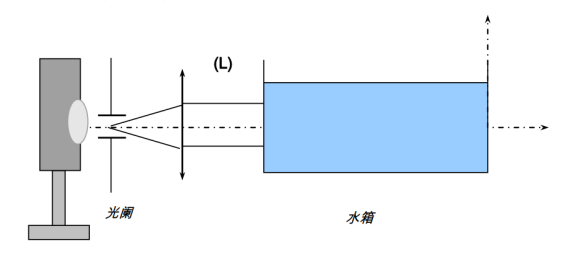
\includegraphics[width=0.6\linewidth]{散射.png}
	
		\label{}
	\end{figure}
	\begin{enumerate}
		\item 实验材料:白光光源, 凸透镜,可变光阑,偏振片P,水槽,奶粉。
		\item 实验步骤
		\begin{enumerate}
			\item 在准直光束产生的平行光中放置水槽,水槽的面相平行。
			\item 倒入少许奶粉(不溢出) 。
			\item 用偏振片观察在(Ox)横向方向的散射光。通过水中倒入的少许粉末的作用,可观察到,在光
			传播垂直方向上,光(部分地) 在垂直方向(Oy)是线性偏振光。
		\end{enumerate}
	\end{enumerate}
	\subsubsection{分析$\lambda/2$波片特性}
\begin{enumerate}
	
	\item $\text{实验器材:氦氖激光器,短焦距透镜,偏振片$P_1$,偏振片$P_2$,}\lambda/2\text{波片,小屏幕。}$
	\item 实验步骤


	\begin{enumerate}
		\item  将偏振片$P_1$和$P_2$放置约20厘米的距离,旋转偏振片找到消光位置。然后将$\lambda/2$波片放在两个
		偏振片之间:观看屏幕,旋转半波片,直到消光重新出现。证明这时有两个相互垂直方向出现消
		光现象。 这时, $\lambda/2$波片的o轴或e轴方向与偏振片P1的偏振方向平行, 确定对应的位置。
		\item 旋转偏振片$P_{1}$ 20度。通过旋转偏振片$P_{2}$, 重新出现消光现象。记录偏振片$P$的位置。证实通过从2半波片的作用,线性偏振光可产生对称o轴或e轴方向的线偏振光。
	\end{enumerate}




\end{enumerate}
\subsubsection{分析$\lambda/4$波片特性}
\begin{enumerate}
	
	\item$\text{实验材料:氦氖激光器,短焦镜头,偏光片P1,偏振片P2,四分之一波片}\lambda/4\text{,小屏幕。}$
	\item 实验步骤


	\begin{enumerate}
		\item  将确定两个偏振片的消光位置。
		\item 将$\lambda/4$波片放置在两个偏振片之间,观察屏幕。\\
		旋转$\lambda/4$波片,直到消光重新出现,确定$\lambda/4$波片对应的位置。说明这时有两个相互垂直方向出现消光现象。证明此时$\lambda/4$片的o轴或e轴方向与偏振片P1的偏振方向平行。
		
	\end{enumerate}




\end{enumerate}
\subsubsection{分析两个$\lambda/4$波片特性}
\begin{enumerate}
	
	\item 实验材料:氦氖激光器,短焦距透镜,光阑,两个偏振片,两个$\lambda/4$ 波片。
	\item 实验步骤
   \begin{enumerate}
		\item  确定两个偏振片的消光位置
		\item 放置第一个$\lambda/4$波片,重现消光现象。记录消光位置。
		\item  再放入第二个$\lambda/4$波片,出现消光时,记录消光的位置。说明这时两个$\lambda/4$波片的o轴或e轴相平行。
		
		\item  旋转$P_1$偏振片20°, 标识旋转的方向。然后旋转偏振片$P_2$重新达到消光,记录偏振片$P_2$的位置。说明此时两个$\lambda/4$波片的关系 (即是两个波片的快慢轴一致?还是一个波片的快轴与另一个波片的慢轴重合?)。
		
		\item  旋转其中一个$\lambda/4$波片90度,再旋转偏振片$P_2$重新达到消光,记录偏振片$P_2$的位置。说明此时两个$\lambda/4$波片的关系。
		
	\end{enumerate}




\end{enumerate}
\subsubsection{研究椭圆偏振光和圆偏振光}
\begin{enumerate}
	
	\item 实验材料:氦氖激光器,短焦距透镜,可变光阑,两个偏振片,四分之一波片$\lambda/4$ 。
	\item 实验步骤
   \begin{enumerate}
		\item  确定两个偏振片的消光位置
		\item 放置第一个$\lambda/4$波片,重现消光现象。旋转$P_1$偏振器片45度,标识旋转方向。旋转偏光片$P_2$,观察屏幕上的光强变化,加以说明。

		\item  再旋转$P_1$。偏振片的角度10度,旋转$P_2$偏光片,观察屏幕上光强的变化。加以说明。
		
		
	\end{enumerate}




\end{enumerate}


	% ---
	
	% 原始数据
	\clearpage
	\subsection{原始数据记录}
	实验记录本上的原始数据见%\cref{}(签字)。
	
	实验台桌面整理见%\textbf{附件}部分(\cref{})。
	
	其它原始数据见%\cref{}。
	% ---
	
	% 问题记录
	\subsection{实验过程遇到问题及解决办法}
	\begin{enumerate}
		\item 
	\end{enumerate}
	% ---
	
	
	
	% 分析与讨论	
	\clearpage
	
	% 顶栏
	\begin{table}
		\renewcommand\arraystretch{1.7}
		\begin{tabularx}{\textwidth}{|X|X|X|X|}
			\hline
			专业:& 物理学 &年级:& 2022级\\
			\hline
			姓名: &  & 学号:& \\
			\hline
			日期:&  & 评分: &\\
			\hline
		\end{tabularx}
	\end{table}
	% ---
	
	% 小标题
	\section{ETX 实验名称××× \quad\heiti 分析与讨论}
	% ---
	
	% 数据处理
	\subsection{实验数据分析}
	
	%
	\subsubsection{}
	\begin{enumerate}
		\item 
	\end{enumerate}
	
	%
	\subsubsection{}
	\begin{enumerate}
		\item 
	\end{enumerate}
	
	%
	\subsubsection{}
	
	% ---
	
	% 实验后思考题
	\subsection{实验后思考题}
	
	%思考题1
	\begin{question}
		
	\end{question}
	
	% 思考题2
	\begin{question}
		
	\end{question}
	
	% 思考题3
	\begin{question}
		
	\end{question}
	
	% ---
	
	
	% 结语部分
	\clearpage
	
	% 小标题
	\section{ETX 实验名称××× \quad\heiti 结语}
	% ---
	
	% 总结、杂谈与致谢
	\subsection{实验心得和体会、意见建议等}
	\begin{enumerate}
		\item 
	\end{enumerate}
	% ---
	

	% 附件
	\subsection{附件及实验相关的软硬件资料等}
	试验台桌面整理如%\cref{}所示。
	
	实验报告个人签名如

	% ---
	
	
\end{document}